\chapter{Stima della matrice di trasformazione}
\label{chap:stima}

\begin{minipage}{12cm}\textit{In questo capitolo verrà trattato il problema della stima della matrice di trasformazione tra due set di coppie di punti. Tale problema, può essere ricondotto ad uno molto antico, noto come problema di Procrustes. Si studieranno due diversi approcci alla soluzione.}
\end{minipage}

\vspace*{1cm}

Come già preannunciato, obbiettivo di questo capitolo è quello di riuscire ad individuare la matrice di trasformazione tra due set di punti. Tali set si suppongono avere la stessa "forma", cioè essere delle grandezze strettamente correlate: ad esempio possono essere campioni della stessa quantità misurati da differenti sensori; oppure essere le coordinate di punti dello spazio in istanti del tempo diversi. Nel seguito si definirà il problema e si studieranno due soluzioni differenti atte a trovare, in forma analitica, la trasformazione in esame.  

%qua descrivo il problema...
\section{Il problema: Superimposizione di Procrustes}
\label{sec:problStima}
Il problema in esame si configura come una versione semplificata di un antico problema detto \textbf{superimposizione di Procrustes}. Nell'antica mitologia greca Procrustes, o Damaste, era un brigante solito aggredire i viaggiatori per poi smembrarli in modo di riuscire disporre le membra su di un tavolo di ferro. 
Per fortuna, il problema matematico in esame risulta meno cruento e può essere riassunto nel modo seguente: \textit{dati due corpi (N-dimensionali), attraverso solo operazioni di rotazione, traslazione e ridimensionamento, si deve riuscire a far combaciare il primo sul secondo in modo ottimo. L'ottimo viene valutato attraverso una quantità detta distanza di Procrustes.} Si dice che il primo viene super-imposto sul secondo; ovviamente qualora i due corpi abbiano la stessa forma la distanza di Procrustes sarà nulla. 
Tale problema risulta molto studiato in ambiti bioinformatici per comparare strutture di proteine. 

Nel resto del capitolo verrà però imposto un vincolo: \textit{i corpi posti a confronto non sono stati scalati.} Tale vincolo, permette di non dover considerare operazioni di ridimensionamento. Infatti, come già preannunciato nel capitolo \ref{chap:visualObs}, l'ambiente circostante si supporrà statico e quindi in nessun modo esso potrà essere ridimensionato.
Inoltre, adotteremo una struttura specifica per i corpi in esame: essi si suppongono essere dei politopi, descritti quindi dai loro vertici. In sostanza questo ci permette di dover tener conto di soli insiemi di punti. 




\section{Il metodo di Groebner}
\label{sec:groeb}
In questo paragrafo si presenta una metodologia di risoluzione del problema in esame mediante l'utilizzo degli strumenti di geometria algebrica. Si procederà prima allo studio del caso planare per poi estendere il risultato al caso spaziale.

\subsection{Il caso planare}
\label{sec:groeb:plan}



\subsection{Il caso spaziale}
\label{sec:groeb:spaz}

%con groebner diretto non si riece a completare il calcolo
Forti della metodologia utilizzata per il caso planare, si è cercato in prima istanza di riprodurla per il caso spaziale. Analogamente a quanto fatto quindi, si è dovuto fissare l'ideale di partenza. 

La prima scelta da effettuare è relativa alla rappresentazione da usare per la matrice di rotazione: si può utilizzare una rappresentazione mediante matrice ortonormale (come fatto nel caso planare), oppure una rappresentazione strutturata. In alcune rappresentazioni, come in forma ortonormale i parametri da stimare sono più numerosi rispetto che con altre, ma ad un maggior numero di parametri corrisponde un aumento del numero dei vincoli. 
Si è scelto di provare con tre differenti rappresentazioni quali forma ortonormale e quaternioni.

Siano: $w_1, w_1^{'}, w_2, w_2^{'}, w_3, w_3^{'} \in \mathbb{R}^3$ rispettivamente i punti omologhi prima e dopo la rotazione per i tre punti considerati, i quali si suppongono noti. Siano $t \in \mathbb{R}^3$ il vettore di traslazione da stimare e $R \in \mathbb{R}^{3 \times 3}$ la matrice di rotazione da stimare. Per ciascuna rappresentazione si può utilizzare il seguente ideale:

\begin{enumerate}
	\item \textbf{Rappresentazione ortonormale}
	 \begin{center}
	 	$M = 
	 	\begin{bmatrix}
	 		r_{11} \, r_{12} \, r_{13} \\
	 		r_{21} \, r_{22} \, r_{23} \\
	 		r_{31} \, r_{32} \, r_{33} 	 	
	 	\end{bmatrix}$\\ \vspace{10pt}
	 	$w_1 - Mw_1^{'}, w_2 - Mw_2^{'}, w_3 - Mw_3^{'}$ \\
	 	$R^{T}R - I$ \\
	 	$det(R) - 1$	 	
	 \end{center}
	\item \textbf{Rappresentazione quaternioni}  
	\begin{center}
		\nonumber $M = 
		\begin{bmatrix}
			2(n^2+e_1^2) - 1 \,\,\, 2(e_1e_2 - ne_3) \,\,\, 2(e_1e_3 + ne_2) \\
			2(e_1e_2+n*e_3) \,\,\, 2(n^2+e_2^2) - 1 \,\,\, 2(e_2e_3 - ne_1) \\
			2(e_1e_3-ne_2) \,\,\, 2(e_2e_3+ne_1) \,\,\, 2(n^2+e_3^2) - 1	 	
		\end{bmatrix}$\\ \vspace{10pt}
		$w_1 -  Mw_1^{'}, w_2 - Mw_2^{'}, w_3 - Mw_3^{'}$ \\
		$e_1^2 + e_2^2 + e_3^2 + w^2 - 1 $
	\end{center}
\end{enumerate}

Purtroppo in tutti e tre i casi riportati il software Macaulay non è stato in grado di portare a termine il calcolo in tempo utile. Infatti, si ricorda che il calcolo di una base di Groebner è un problema EXPSPACE-completo. 

%estendo 2d
Si è ritenuto allora che fosse più istruttivo un cambio di approccio.
\begin{pro}
	data la soluzione del problema planare, è possibile estenderla al caso spaziale?
\end{pro}

In effetti, attraverso qualche ragionamento di natura geometrica, è stata possibile tale estensione. Di seguito si descrive l'approccio usato.

% porto centroidi su origine
\begin{defn}
	Si consideri un set di punti $\left\lbrace w_1, w_2, ..., w_N \right\rbrace$, si definisce \textbf{punto centroide} il punto centrale del set, calcolato come media puntuale dei punti.
	\begin{equation}
		w_c = \frac{1}{N}\sum_{i = 1}^{N} w_i
	\end{equation}
\end{defn}

Occorre considerare almeno tre coppie di punti omologhi $(w_i, w_i^{'})$ (ciascuna coppia è costituita dal i-esimo punto prima e dopo la rotazione). Si costruiscano allora due set di punti $W = \left\lbrace w_1, w_2, w_3 \right\rbrace$ e $W = \left\lbrace w_1^{'}, w_2^{'}, w_3^{'} \right\rbrace$

Per ciascuno dei due set si calcoli il suo punto centroide $w_c$ e $w_c^{'}$ rispettivamente.

In prima istanza occorre traslare i due set di punti in modo che il punto centroide coincida con l'origine. Per fare ciò possiamo semplicemente sottrarre il punto centroide ai punti del relativo set.
\begin{equation}
p_i = w_i - w_c, \, \, 
p_i^{'} = w_i - w_c^{'}
\end{equation}
dove per comodità di notazione si sono definiti con la lettera "p" i punti al netto di tale operazione.

% individuo asse mozzi
\begin{defn}
	Sia considerata una trasformazione (rotazione e traslazione) di un set di punti, si definisce \textbf{asse dei mozzi}, l'asse i cui punti, durante la trasformazione, subiscono una sola traslazione lungo lo stesso. 
\end{defn}

\begin{obs}
	\label{rot:gb:mozzi}
	In caso di una sola rotazione lungo un asse passante per l'origine l'asse dei mozzi coincide con l'asse di rotazione stesso.
	
	Inoltre se si considerano tre coppie di punti omologhi, l'asse dei mozzi può essere calcolato come l'intersezione dei due piani definiti dai tre punti appartenenti a tali coppie rispettivamente prima e dopo la rotazione.
\end{obs}

Grazie al fatto che abbiamo traslato i punti in modo tale di far coincidere i centroidi nell'origine, vale l'osservazione \ref{rot:gb:mozzi}.

Possiamo calcolare pertanto l'asse dei mozzi come l'intersezione dei piani definiti dai set $P$ e $P^{'}$. Nella figura \ref{rot:gb:imgMozzi} si può evincere più facilmente quanto detto.
\begin{figure}[h]
	\centering
	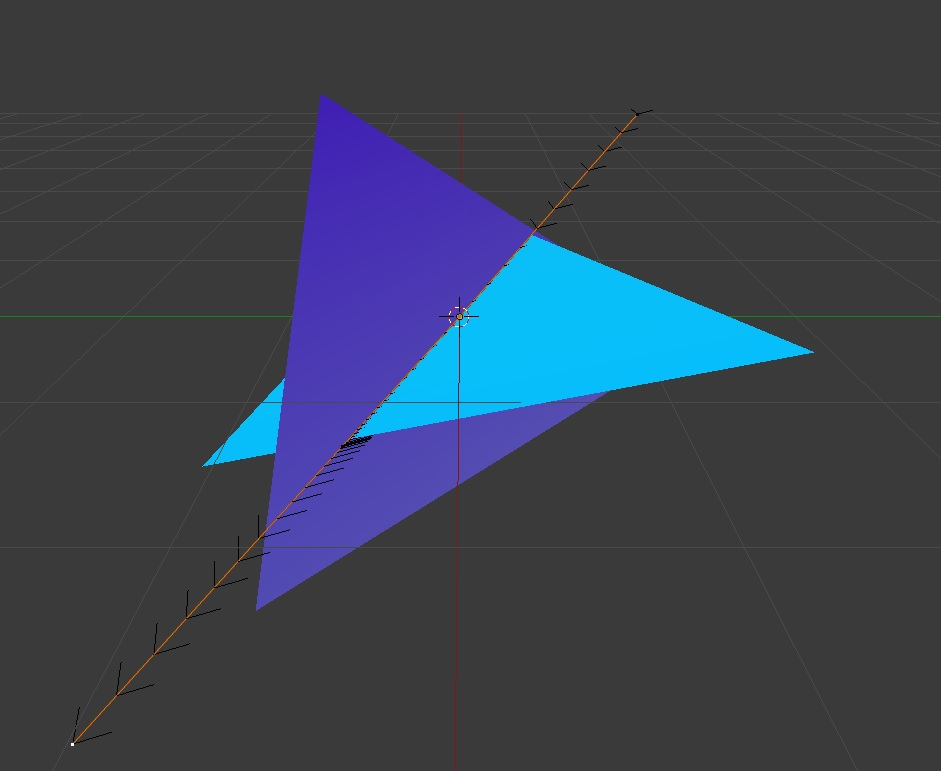
\includegraphics[width=420pt]{imgs/AsseMozzi.jpg}
	\caption{Calcolo dell'asse dei mozzi attraverso intersezione dei piani omologhi}
	\label{rot:gb:imgMozzi}
\end{figure} 

% rotazione su asse dei mozzi
% rotazione 2d nel piano dei punti
% rotazione totale come motliplicazione delle due matrici di rotazione risultanti.
\section{Il metodo di Kabsch}
\label{sec:kabsch}

Nel precedente paragrafo si è riusciti ad individuare una soluzione in forma chiusa per il problema in esame; tale soluzione faceva uso di un numero molto ridotto di punti omologhi per il calcolo ma un possibile errore o rumore sui set faceva si che le prestazioni della stima degenerassero.

Si presenta ora una soluzione in grado di individuare la trasformazione ottima tra i due set di punti, più robusta al rumore.

Questo metodo è stato presentato per la prima volta in \cite{bib1} ad opera di W. Kabsch, in una prima formulazione si faceva uso del concetto di moltiplicatori di Lagrange, i quali avevano un impatto prestazionale abbastanza elevato. In questa recente formulazione invece si utilizza la decomposizione SVD, strumento il cui calcolo negli ultimi anni è diventato molto efficiente.

La trasformazione che vogliamo individuare è composta, ovviamente, da una rotazione e una traslazione. Conviene iniziare con l'individuazione della prima, ragionando in modo analogo al precedente paragrafo, si comincia con il calcolo dei centroidi. Per comodità si riporta la formula per il calcolo del centroide di un set di punti:
\begin{equation}
	\label{rot:eq:cent}
	a_c = \frac{1}{N}\sum_{i = 1}^{N}a_i
\end{equation}
Si procede poi traslando i set di punti facendo si che i centroidi coincidano con l'origine:
\begin{equation}
\label{rot:eq:redef}
a_i^{'} = a_i - a_c, \, \, 
b_i^{'} = b_i - b_c
\end{equation}

Il problema ora può essere formulato come un problema di controllo ottimo: \textit{trovare la matrice ortonormale $R$ tale che la distanza di Procrustes tra i due set sia minima.} Grazie al fatto che i centroidi dei due set coincidono, tale distanza, ridefinendo come $x_i = a_i^{'}, y_i = b_i^{'}, x_i, y_i \in \mathbb{R}^d$ per comodità, può essere calcolata semplicemente come:
\begin{equation}
	\label{rot:eq:dist}
	d(x, y) =  \frac{1}{N}\sum_{i = 1}^{N} \| R x_i - y_i \|^2
\end{equation}
Si fissa quindi l'indice di costo $J = d(x, y)$. 
Si fa notare che imporre la sola ortonormalità della matrice $R$ non assicura che essa sia una matrice di rotazione propria. Infatti si dovrà fare in modo che il suo determinante sia pari a 1. In caso contrario (pari a -1) essa rappresenterebbe una rotazione impropria, cioè una componente dei punti risulterebbe "specchiata". 
Si possono rappresentare i set di punti attraverso le matrici:
\begin{equation}
	X = [x_1 \, x_2 \, ... \, x_N], Y = [y_1 \, y_2 \, ... \, y_N], X, Y \in \mathbb{R}^{d \times N},
\end{equation}
e sia $X^{'} = RX, \, \, X^{'} = [x_1^{'} \, x_2^{'} \, ... \, x_N^{'}]$ la matrice dei punti ruotati.

Possiamo allora scrivere che:
\begin{equation}
	N J = \sum_{i = 1}^{N} \| x_i^{'} - y_i \|^2 = Tr[(X^{'} - Y)^{T}(X^{'} - Y)]
\end{equation}
dove si indica con $Tr(A)$ l'operatore traccia della matrice $A$.
Grazie alla linearità dell'operatore traccia vale che:
\begin{equation}
Tr[(X^{'} - Y)^{T}(X^{'} - Y)] = Tr(X^{'T}X^{'}) + Tr(Y^{T}Y) - 2Tr(Y^{T}X^{'})
\end{equation}
Inoltre vale l'identità:
\begin{equation}
\label{rot:eq:mod}
Tr(X^{'T}X^{'}) + Tr(Y^{T}Y) = \frac{1}{N}\sum_{i = 1}^{N} \| x_i^{'} \| ^ 2 + \| y_i \| ^ 2
\end{equation}
In seguito alla (\ref{rot:eq:redef}) i punti di entrambi i set sono dei vettori centrati nell'origine. La rotazione di un vettore non può in nessun modo alterarne il suo modulo. Si può affermare allora che la quantità (\ref{rot:eq:mod}) è costante e può essere non considerata nella minimizzazione dell'indice. Pertanto, per minimizzare il suddetto indice, basterà massimizzare la quantità $Tr(Y^{T}X^{'}) = Tr(Y^{T}RX) = Tr((XY^{T})R)$.
Si fa notare che la matrice $ C = XY^{T}, \, C \in \mathbb{R}^{d \times d}$ è la matrice di cross correlazione tra i due set.

Si usa ora la decomposizione SVD della matrice $C = VSW^T$, si ha che $V, S, W^T \in \mathbb{R}^{d \times d}$ poiché $C$ è quadrata. La matrice $S$ è diagonale e i suoi elementi sono i valori singolari della matrice $C$ in ordine decrescente.
Dato che per l'operatore traccia vale che $Tr(AB) = Tr(BA)$, indicando con $A = V$ e $B = SW^TR$ è possibile scrivere:
\begin{equation}
	Tr(Y^{T}X^{'}) = Tr(VSW^TR) = Tr(SW^TRV) = \sum_{i = 1}^{d} s_iw_i^TRv_i
\end{equation}
La matrice $T = W^TRV$ è il prodotto di matrici ortonormali, sarà anch'essa ortonormale, questo vuol dire che i suoi elementi non potranno avere modulo maggiore di 1. Pertanto indicando con $T_{ii} = w_i^TRv_i$ gli elementi sulla diagonale di $T$, vale che
\begin{equation}
	Tr(Y^{T}X^{'}) = \sum_{i = 1}^{d} s_iT_{ii} \leq \sum_{i = 1}^{d} s_i
\end{equation}
 pertanto al massimo il valore della quantità $Tr(Y^{T}X^{'})$ è pari alla somma dei valori singolari $s_i$. Si deve fare in modo quindi che la matrice $T$ sia una matrice identità.
 Grazie alla proprietà di $V$ e $W^T$ di essere ortonormali, $VV^T = I, W^TW = I$, basterà scegliere:
 \begin{equation}
 	R = WV^T
 \end{equation}
Resta da risolvere un problema, cioè che in generale $det(R) = \pm 1$, il caso negativo va evitato.
Per fare ciò possiamo aggiungere il vincolo che $det(R) = 1$ al problema, ripercorrendo quanto fatto e notando che $s_1 \ge s_2 \ge \, ... \, \ge s_d$ e che
\begin{equation}
Tr(Y^{T}X^{'}) = \sum_{i = 1}^{d} s_iT_{ii} 
\end{equation}
possiamo individuare il massimo per questa quantità, rispettando il vincolo, con la scelta $T_{11} = T_{22} = \, ... \, = T_{d-1d-1} = 1, T_{dd} = -1$. Infatti, data la richiesta di ortonormalità deve valere che i $T_{ii}$ devono essere in modulo pari a 1, quindi quest'ultima è la scelta migliore possibile dato che si sottrae il valore singolare più piccolo. Basterà dunque in caso di determinante negativo, cambiare di segno all'ultimo vettore singolare destro di $W$ (l'ultima colonna della matrice $W$). Possiamo generalizzare i due casi cosi facendo:
\begin{equation}
	d = sign(det(WV^T)),
\end{equation}
\begin{equation}
	R = W
	\begin{bmatrix}
	1 \,\, 0 \,\, \cdots \,\, 0\\
	0 \,\, 1 \,\, \cdots \,\, 0\\
	\vdots\\
	0 \,\, \cdots \,\, 1 \,\, 0\\
	0 \,\, \cdots \,\, 0 \,\, d\\
	\end{bmatrix}V^T
\end{equation}

Trovata la matrice di rotazione ottima, relativa ai due set, si può procedere ad individuare il vettore di traslazione relativo tra i due set. Si procede in maniera del tutto analoga a quanto fatto nel paragrafo \ref{sec:groeb:spaz} e per comodità si riporta qui la formula:
\begin{equation}
	t = b_c - Ra_c, t \in \mathbb{R}^d
\end{equation}
dove $b_c$ e $a_c$ sono i centroidi precedentemente calcolati.
\subsection{Robustezza ai disturbi}
\label{sec:kabsch:rumore}
La soluzione appena ottenuta, come preannunciato, oltre che ottima, risulta resistente a disturbi sulla misura. Infatti, si supponga il disturbo "bianco", cioè con valore atteso pari a 0 e il disturbo delle singole componenti indipendente dalle altre.

In prima istanza si può notare che il calcolo dei centroidi risulta corretto a patto di utilizzare un numero "abbastanza" grande di misure. Infatti, considerando $\tilde{x_i}$ la i-esima misura disturbata, si ha che
\begin{equation}
	x_c = \frac{1}{N}\sum_{i = 1}^{N} \tilde{x_i} = \frac{1}{N}\sum_{i = 1}^{N} x_i + e_i \longrightarrow \hat{x} + E[e] = \hat{x}
\end{equation}
dove con $E[e]$ si indica il valore atteso del disturbo. Dove nella precedente relazione la probabilità di convergenza ri al crescere delle misure disponibili, grazie alla legge dei grandi numeri: 
